\chapter{Incoherency} \label{chap:Incoherency}

In this chapter the blending operator is analyzed in greater detail. The analysis aims to propose a blending operator, which facilitates better deblending. Before starting the analysis I will introduce a new measure of incoherency. Then, I will discussed how incoherency and the so-called maximum firing-time delay influence deblending.

\section{Analysis of the Blending Matrix} \label{sec:BlendingMatrix}

In order to optimize the blended-acquisition design, one must understand the properties of the blending matrix, $\mathbf{\Gamma}$, and its influence on the deblending performance.

The blending matrix, $\mathbf{\Gamma}$, determines the pseudo-deblended data,

\begin{equation}
	\mathbf{P}_{ps} = \mathbf{P \Gamma \Gamma}^H,
	\label{eq:Ch-Theory-Pseudo-Deblended-Data}
\end{equation}

which are a superposition of the unblended data, $\mathbf{P}$, and the blending noise, $\mathbf{N}$,

\begin{equation}
	\mathbf{P}_{ps} = \mathbf{P} + \mathbf{N} = \mathbf{P I} + \mathbf{P} \; (\mathbf{\Gamma \Gamma}^H - \mathbf{I}).
	\label{eq:Ch-Theory-PseudoSuperposition}
\end{equation}

The more incoherent the blending noise, $\mathbf{N}$, the better it can be estimated with the coherency constraint presented in chapter \ref{chap:theory}.

In the following the effect of the blending matrix, $\mathbf{\Gamma}$, on the pseudo-deblended data, $\mathbf{P}_{ps}$, is analyzed. For simplicity, it is assumed that all shots are equal in strength and fire the same signature into the earth. It is also assumed that each shot is fired only once, unlike e.g. the shot repetition case \citep{Sixue}. This means that the blending matrix, $\mathbf{\Gamma}$, only contains phase shift terms, $\mathrm{e}^{-j \omega \Delta t}$, or zeros. The phase shift terms , $\mathrm{e}^{-j \omega \Delta t}$, are defined by the firing-time delay between blended shots, $\Delta t$. 
\nomenclature{$\omega$}{Circular frequency}

Each row of $\mathbf{\Gamma}$ represents a shot $k$, and each column of $\mathbf{\Gamma}^H$ represents a shot $l$ with a complex conjugated phase term (see Figure \ref{fig:Ch-Theory-GGH}). Hence, each element of the matrix product $\mathbf{\Gamma \Gamma}^H$, $g_{kl}$, is the dot product between the $k^{th}$ shot and the complex conjugate of the $l^{th}$ shot.

\begin{figure}
	\centering
	\includegraphics[width = \textwidth]{Plots/GGH_v2}
	\caption{Illustration of the matrix product, $\mathbf{\Gamma \Gamma}^H$. In this notation $\Delta t_k$ refers to the phase shift of the shot $k$, and $\Delta t_{kl}$ refers to the phase shift between the shots $k$ and $l$, $\Delta t_{kl} = \Delta t_k - \Delta t_l$.}
	\label{fig:Ch-Theory-GGH}
\end{figure}

Consequently, an element $g_{kl}$ of the matrix product, $\mathbf{\Gamma \Gamma}^H$, represents the overlap of the shots $k$ and $l$ for all experiments. The main diagonal of $\mathbf{\Gamma \Gamma}^H$ refers to the overlap of each shot with itself, which of course is perfect and therefore equal to 1. The off-diagonal elements of $\mathbf{\Gamma \Gamma}^H$ are either 0 if the associated shots do not overlap, or contain a phase shift, $\mathrm{e}^{\, -j \omega \Delta t_{kl}}$.

\subsection*{Temporal incoherency}

In the following the term "sub-diagonal" will be used to refer to an arbitrary diagonal of the matrix $\mathbf{\Gamma \Gamma}^H$. For example, the $d^{th}$ sub-diagonal includes all the matrix elements $g_{ij}$\nomenclature{$g_{ij}$}{Element of the matrix product $\mathbf{\Gamma \Gamma}^H$ corresponding to the interference between the $i^{th}$ and $j^{th}$ source}, which fulfill the condition; $j -i = d$.

In equation \ref{eq:Ch-Theory-PseudoSuperposition} the main diagonal elements of $\mathbf{\Gamma \Gamma}^H$ copy the data matrix, $\mathbf{P}$, while the off-diagonal elements create the blending noise, $\mathbf{N}$. In case of constant firing-time delays the elements along a sub-diagonal $d$ all have the same phase. This means that the sub-diagonal elements will shift the columns of the data matrix and apply a constant phase shift to each of them resulting in the pseudo-deblended receiver gather shown in Figure \ref{fig:Ch-Theory-PseudoCRG-CoherentDelay}. If the firing-times are random instead of constant, the elements $g_{ij}$ along a sub-diagonal $d$ will have different phases. Consequently, they will shift the columns of the data matrix, and distort the phase of each column (see Figure \ref{fig:Ch-Theory-PseudoCRG-IncoherentDelay}). 

Figure \ref{fig:Ch-Theory-PseudoCRG-FK-CoherentDelay} and \ref{fig:Ch-Theory-PseudoCRG-FK-IncoherentDelay} display the $f$-$k$ spectra of the pseudo-deblended data for constant firing-time delays and random firing-time delays respectively. In the case of constant firing-time delays all of the energy maps in the signal cone. In the case of random firing-time delays a significant part of the energy maps outside of the signal cone. From Figure \ref{fig:Ch-Theory-PseudoCRG-FK-CoherentDelay} and \ref{fig:Ch-Theory-PseudoCRG-FK-IncoherentDelay} it is clear that the coherency constraint presented in section \ref{sec:IterBlenNoiseEst} cannot work with constant firing-time delays, but needs the random firing-time delays. 

In this thesis the random firing-time delays along a sub-diagonal are referred to as temporal incoherency.  

\begin{figure}
	\centering
	\begin{subfigure}[b]{0.3\textwidth}
		\centering
		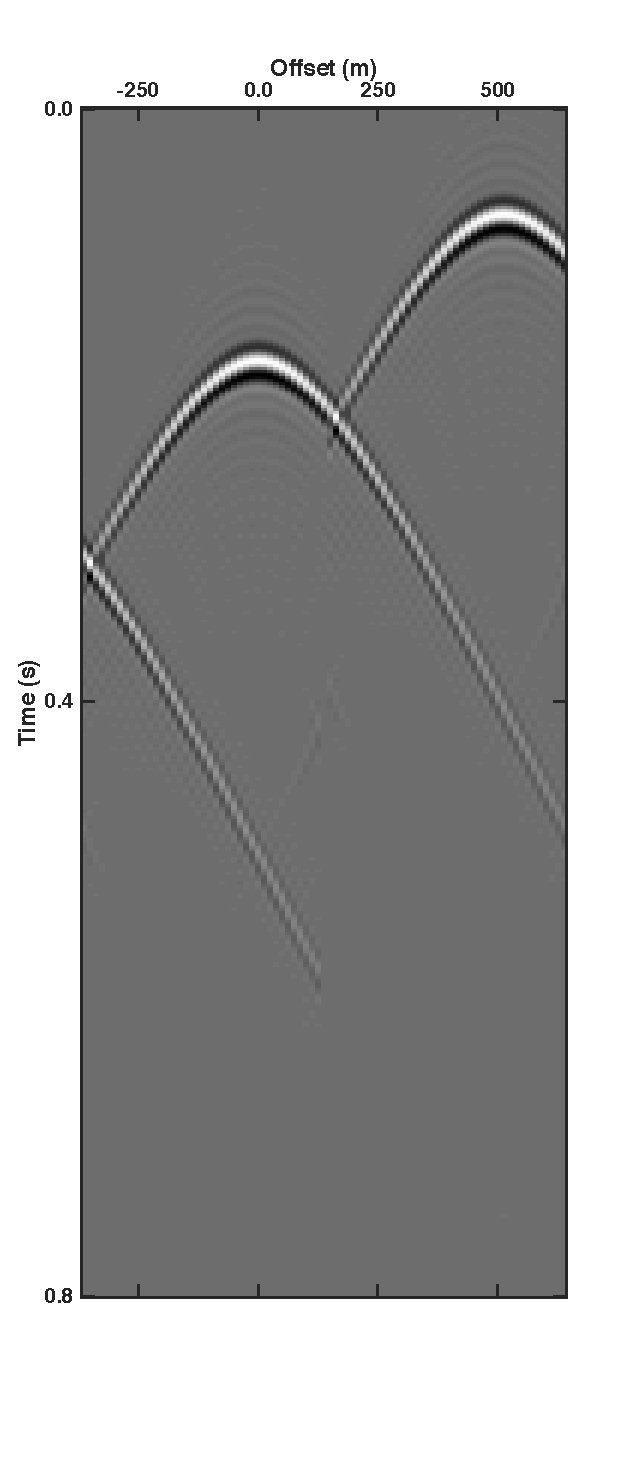
\includegraphics[width = \textwidth]{Plots/Mahdad/25iter/TimeDelay/Pseudo-DeblendedCRG_rec30_coh}
		\caption{}
		\label{fig:Ch-Theory-PseudoCRG-CoherentDelay}
	\end{subfigure}
	%
	\centering
	\begin{subfigure}[b]{0.3\textwidth}
		\centering
		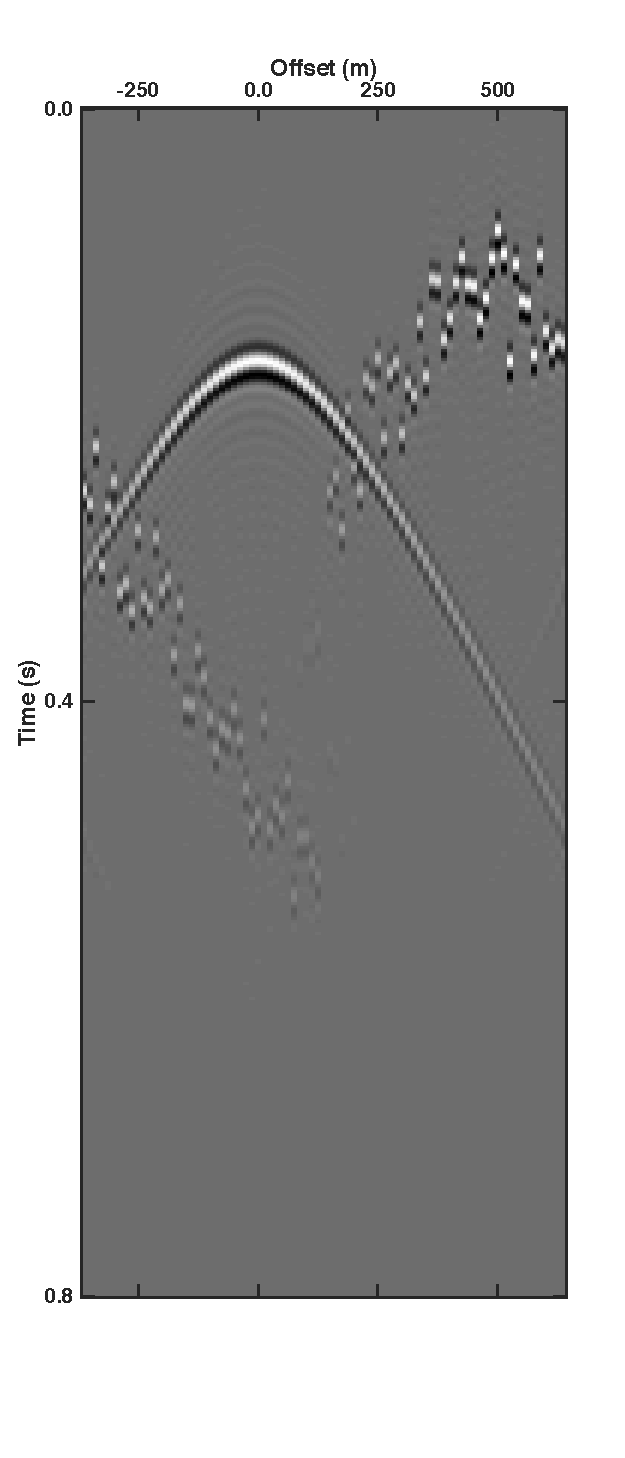
\includegraphics[width = \textwidth]{Plots/Mahdad/25iter/TimeDelay/Pseudo-DeblendedCRG_rec30}
		\caption{}
		\label{fig:Ch-Theory-PseudoCRG-IncoherentDelay}
	\end{subfigure}
	%
	\centering
	\begin{subfigure}[b]{0.3\textwidth}
		\centering
		\includegraphics[width = \textwidth]{Plots/Mahdad/25iter/Space/Pseudo-DeblendedCRG_rec30_X}
		\caption{}
		\label{fig:Ch-Theory-PseudoCRG-IncoherentSpace}
	\end{subfigure}

	\centering
	\begin{subfigure}[b]{0.3\textwidth}
		\centering
		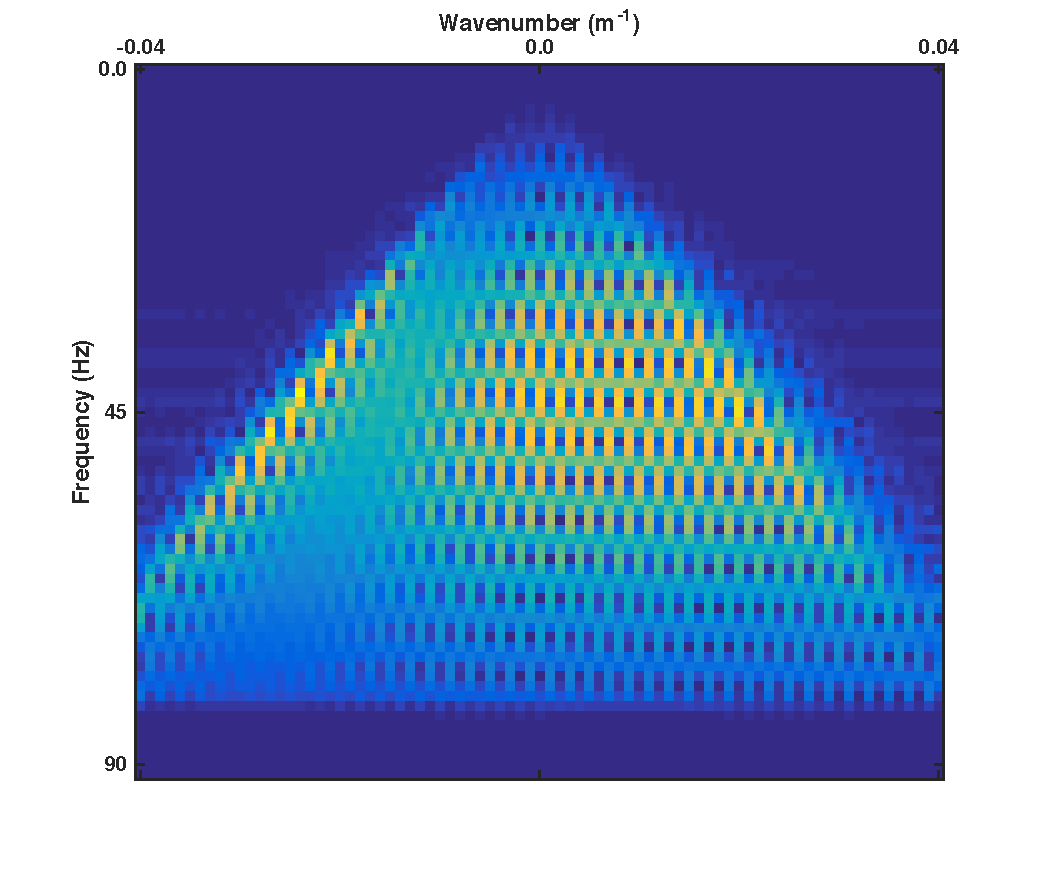
\includegraphics[width = \textwidth]{Plots/Mahdad/25iter/TimeDelay/FK-Pseudo-deblendedCRG_rec30_coh}
		\caption{}
		\label{fig:Ch-Theory-PseudoCRG-FK-CoherentDelay}
		
	\end{subfigure}
	%
	\centering
	\begin{subfigure}[b]{0.3\textwidth}
		\centering
		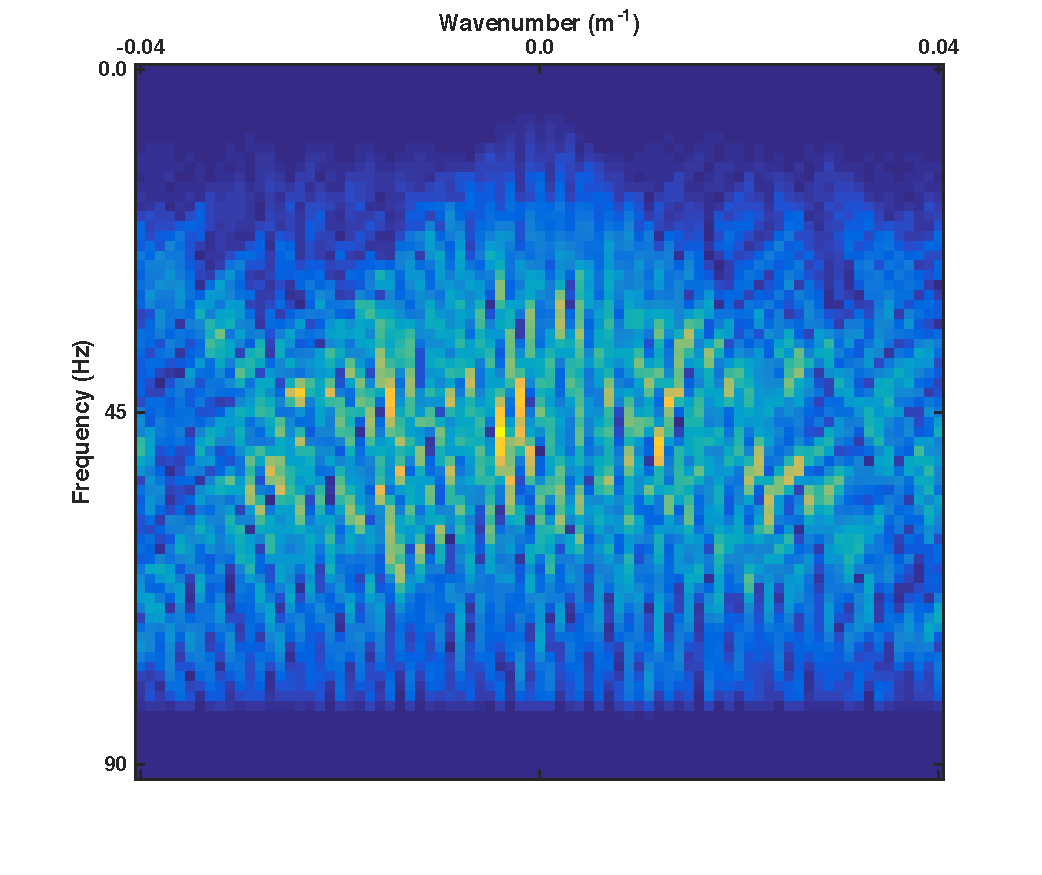
\includegraphics[width = \textwidth]{Plots/Mahdad/25iter/TimeDelay/FK-Pseudo-deblendedCRG_rec30}
		\caption{}
		\label{fig:Ch-Theory-PseudoCRG-FK-IncoherentDelay}
	\end{subfigure}
	%
	\centering
	\begin{subfigure}[b]{0.3\textwidth}
		\centering
		\includegraphics[width = \textwidth]{Plots/Mahdad/25iter/Space/FK-Pseudo-deblendedCRG_rec30_X}
		\caption{}
		\label{fig:Ch-Theory-PseudoCRG-FK-IncoherentSpace}
	\end{subfigure}
	
	\caption{Comparison of the pseudo-deblended receiver gather for (a) constant firing-time delays of \SI{100}{\milli\second}, (b) random firing-time delays between \SI{0}{\milli\second} and \SI{100}{\milli\second} and (c) a spatially incoherent blending pattern. (d) - (f) show the $f$-$k$ spectra of (a), (b) and (c) respectively.}
	\label{fig:Ch-Theory-PseudoCRG-IncoherencyEffect}

\end{figure}

\begin{figure}
	\centering
	\includegraphics[width=\textwidth]{Plots/GGH_x_v2}
	\caption{The blending matrix, $\mathbf{\Gamma}$, is obtained by interchanging the $3^{rd}$ and $4^{th}$ row of the blending matrix in Figure \ref{fig:Ch-Theory-GGH}. In acquisition this is equivalent to moving shot 3 to experiment 2, and shot 4 to experiment 1. A random permutation of the rows of the blending matrix spreads the off-diagonal elements of the matrix product, $\mathbf{\Gamma\Gamma}^H$. The elements are not assembled on the sub-diagonals anymore.}
	\label{fig:Ch-Theory-GGHx}
\end{figure}

\begin{comment}
In order to generate incoherent source interference, $\mathbf{N}$, it is therefore favorable if the elements $a_{ik}$ of each lower or upper diagonal are out of phase. For example, considering the $n^{th}$ upper or lower diagonal of the matrix $\mathbf{\Gamma \Gamma}^H$ this observation translates to the acquisition as follows: All source pairs, which are $n$ sources apart from each other, must be fired incoherently. The incoherent firing is realized by delaying blended sources with a random time delay.
\end{comment}


\subsection*{Spatial incoherency}

Of course, the degree of incoherency of the blending noise, $\mathbf{N}$, also depends on whether the shot positions of shots blended in an experiment are selected spatially in a random or coherent pattern. For example, one expects the blending noise to be more incoherent, if in each experiment randomly selected shot positions are blended as in Figure \ref{fig:Ch-Theory-GGHx}, than if in each experiment adjacent shot positions are blended as in Figure \ref{fig:Ch-Theory-GGH}, because the interfering shots are spread over the sub-diagonals in Figure \ref{fig:Ch-Theory-GGHx}.

In this thesis selecting random shots for an experiment is referred to as spatial incoherency. Figure \ref{fig:Ch-Theory-PseudoCRG-IncoherentSpace} shows a pseudo-deblended common-receiver gather of a blended dataset, which was acquired in a spatially incoherent fashion, i.e. the blended shot-positions are selected randomly but the firing-time delay is always 0. The corresponding $f$-$k$ spectrum is shown in Figure \ref{fig:Ch-Theory-PseudoCRG-FK-IncoherentSpace}.

Although examples of spatial incoherency are shown in this chapter, it has to be noted that to blend shots in a spatially incoherent fashion is not very practical in 2D acquisition. However, in chapter \ref{chap:MahdadMethod3d} it will be shown, that for 3D blending spatial incoherency becomes practical.


\begin{comment}

In terms of the blending matrix $\mathbf{\Gamma}$ a spatially incoherent firing pattern means that the rows, i.e. the sources, are shuffled randomly. As a consequence the off-diagonal elements of the matrix product $\mathbf{\Gamma \Gamma}^H$ are reordered randomly. This shuffling process can help to further distort the phase of the interfering sources. However, if the maximum allowed time delay between blended sources is aready large the spatially incoherent blending pattern will not increase the incoherency of the interfering sources.   

In practice, the maximum allowed firing time delay is limited by the available acquisition time. The spatial distribution of blended sources is constraint by the acquisition design.
	
\end{comment}


\FloatBarrier

\section{Results Spatial and Temporal Incoherency}

Based on the blending matrices in Figure \ref{fig:Ch-Theory-GGH} and \ref{fig:Ch-Theory-GGHx} there are three possibilities to blend the shots incoherently. First, the phase terms along the sub-diagonals can be randomly varied, i.e. the shots are blended with random firing-time delays (temporal incoherency). Second, the rows of the blending matrix can be randomly permuted, i.e. one randomly selects shots for each experiment and fires them with no delay time (spatial incoherency). Third, temporal and spatial incoherency can be combined (mixed incoherency), i.e. randomly selected shots are blended with random firing-time delays.

These 3 blending patterns are applied to a synthetic dataset. The data are a common-receiver gather with 21 shots (see Figure \ref{fig:Ch-Results-Unbl-inline10}), which are blended in 3 experiments with 7 shots per experiment. Next, the data are deblended with the deblending algorithm of section \ref{sec:MahdadMethod}. 

The deblended receiver gathers are shown in Figure \ref{fig:Ch-Results-Debl-x-inline}. The results suggest that only spatial incoherency is not sufficient to deblend the data (see Figure \ref{fig:Ch-Results-Debl-inline10-x}). By introducing random firing-time delays the deblended data improve significantly as shown in Figure \ref{fig:Ch-Results-Debl-inline10-t}. A combination of both spatial and temporal incoherency enhances the deblended data further (see Figure \ref{fig:Ch-Results-Debl-inline10-xt}).

Note that the blending noise in the pseudo-deblended common-receiver gathers in Figure \ref{fig:Ch-Results-Debl-inline10-x} and \ref{fig:Ch-Results-Debl-inline10-t} has a very different spreading. In the case of temporal incoherency the blending noise is spread over a significantly larger time window than in the case of spatial incoherency. This explains why temporally incoherent blending yields superior deblending results.


\begin{figure}
	\centering
	\begin{subfigure}[t]{0.16\textwidth}
		\centering
		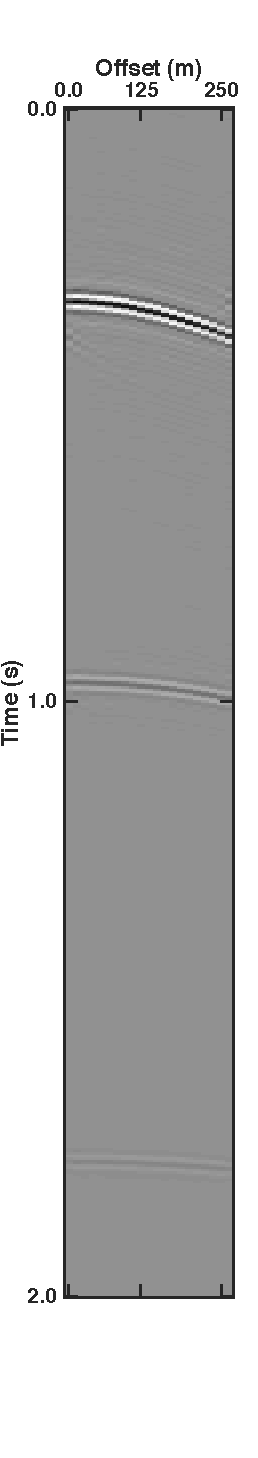
\includegraphics[height = 0.38\textheight]{Plots/BlendingPatterns/Unblended_xline10}
		\caption{}
		\label{fig:Ch-Results-Unbl-inline10}
	\end{subfigure}
	%	
	\centering
	\begin{subfigure}[t]{0.26\textwidth}
		\centering
		\includegraphics[height = 0.38\textheight]{Plots/BlendingPatterns/Pseudo_Deblended_xline10_x_b7}
		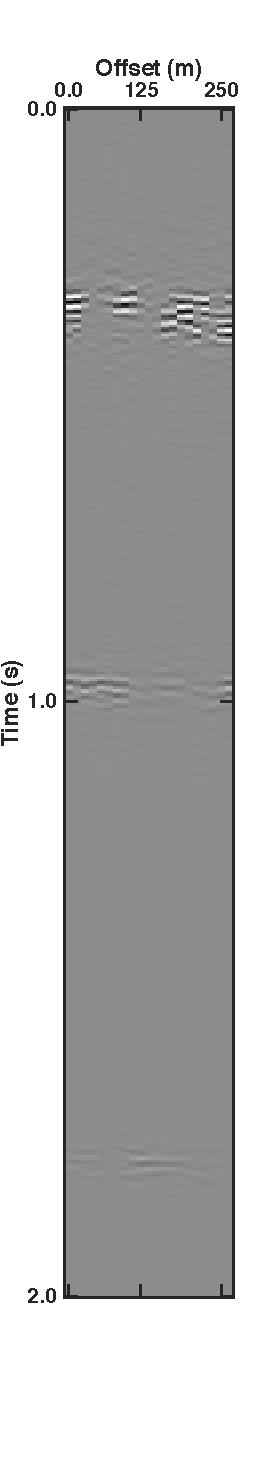
\includegraphics[height = 0.38\textheight]{Plots/BlendingPatterns/Deblended_xline10x}
		\caption{}
		\label{fig:Ch-Results-Debl-inline10-x}
	\end{subfigure}
	%
	\centering
	\begin{subfigure}[t]{0.26\textwidth}
		\centering
		\includegraphics[height = 0.38\textheight]{Plots/BlendingPatterns/Pseudo_Deblended_xline10_t_b7}
		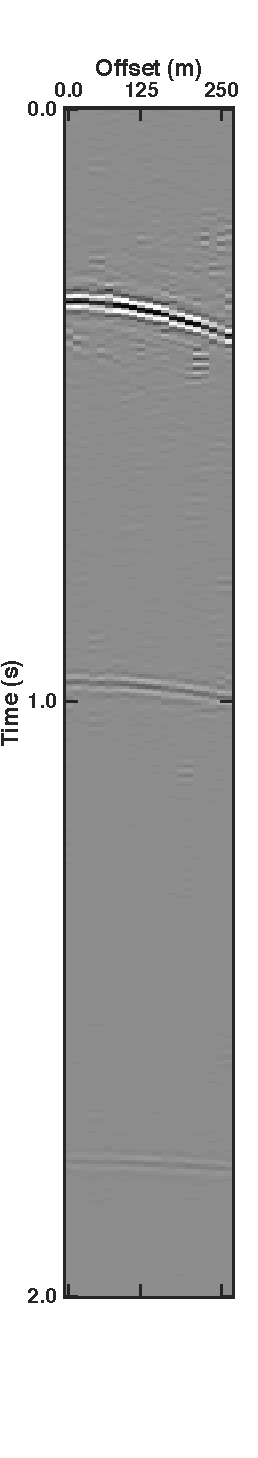
\includegraphics[height = 0.38\textheight]{Plots/BlendingPatterns/Deblended_xline10t}
		\caption{}
		\label{fig:Ch-Results-Debl-inline10-t}
	\end{subfigure}
	%
	\centering
	\begin{subfigure}[t]{0.26\textwidth}
		\centering
		\includegraphics[height = 0.38\textheight]{Plots/BlendingPatterns/Pseudo_Deblended_xline10_xt_b7}
		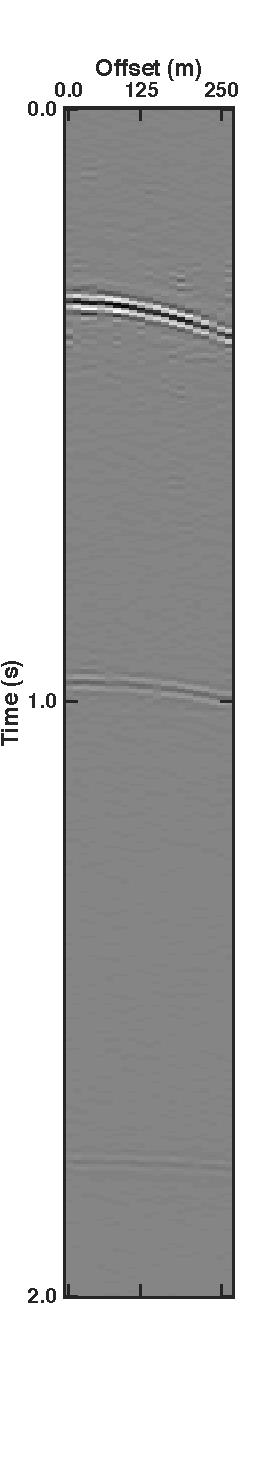
\includegraphics[height = 0.38\textheight]{Plots/BlendingPatterns/Deblended_xline10xt}
		\caption{}
		\label{fig:Ch-Results-Debl-inline10-xt}
	\end{subfigure}
	
	\caption{(a) shows a synthetic unblended common-receiver gather. The data are blended with a (b) spatially incoherent, (c) temporally incoherent, and (d) mixed incoherent blending pattern. The respective pseudo-deblended data (left) and deblended data (right) are shown in (b) to (d).}
	\label{fig:Ch-Results-Debl-x-inline}

\end{figure}


\FloatBarrier
\section{Effect of Incoherency} \label{sec:Effect-of-Incoherency}

This section aims to analyze how strongly the deblending result depends on the incoherency of the blended acquisition. For this purpose I will introduce a measure of incoherency and deblending quality.

\subsection*{Incoherency Measure}

%\todo[inline]{Move this sentence to the introduction (literature). You might also want to mention the work of the Greek guy Apostolos.\\
%In this thesis only the incoherency of the acquisition design is considered. Thus, the blending matrix, $\Gamma$, or more precisely the product $\mathbf{\Gamma \Gamma}^H$ determines the incoherency.}

%A measure of incoherency will be introduced in order to analyze the importance of an incoherent blending pattern quantitatively.

In section \ref{sec:BlendingMatrix} it was shown that for an incoherent blending pattern the elements, $\mathrm{e}^{-j \omega \Delta t_{kl}}$, along a sub-diagonal of the matrix product, $\mathbf{\Gamma \Gamma}^H$, should be out of phase, i.e. each element should contain a different time delay, $\Delta t$. Therefore, the phase variability of the sub-diagonal elements will be used to quantify incoherency. 

\begin{figure}
	\centering
	\includegraphics[width = 0.35\textwidth]{Plots/ComplexPlane}
	\caption{Illustration of the sub-diagonal elements in the complex number plane. The elements have unit length and variable phase. The absolute value of their sum depends on the phase coherency of the elements.}
	\label{fig:Ch-Results-complex-circle}
\end{figure}

The sub-diagonal elements, $\mathrm{e}^{-j \omega \Delta t_{kl}}$, map in the complex plane on a circle with radius 1 (see Figure \ref{fig:Ch-Results-complex-circle}). Thus, the sum of the elements along the $d^{th}$ sub-diagonal can be constructive or destructive (as in the case of Figure \ref{fig:Ch-Results-complex-circle}), depending on the phase variability. The absolute value of this sum, $M(d,\omega)$, measures the incoherency of the $d^{th}$ sub-diagonal for the frequency component, $\omega$;
\nomenclature{$M$}{Absolute value of the sum along a sub-diagonal of the matrix product $\mathbf{\Gamma \Gamma}^H(\omega)$}

\begin{equation}
	M(d,\omega) = \left| \sum_{j-i=d} \mathbf{\Gamma \Gamma}^H_{ij} (\omega) \right|.
	\label{eq:Ch-Results-incoherency-diagsum}	
\end{equation} 

If all sub-diagonal elements are in phase the absolute value of their sum, $M(d,\omega)$, is maximized. Instead, in case of an incoherent blending pattern $M(d,\omega)$ is small for all sub-diagonals $d$, except for the main diagonal ($d = 0$).  

The incoherency measure, $\mu$, is introduced as;

\begin{equation}
	\mu = \frac{\left( \; \sum_{\omega}M(d=0,\omega) \; \right)^2}{\sum_{d = 1-Ns}^{Ns-1} \left(\left( \; \sum_{\omega}M(d,\omega) \; \right)^2\right)} \; ,
	\label{eq:Ch-Results-incoherency}
\end{equation}
\nomenclature{$\mu$}{Incoherency value of the blending matrix $\mathbf{\Gamma}$}

where $N_s$\nomenclature{$N_s$}{Total number of sources} is the number of sources, i.e. the matrix $\mathbf{\Gamma \Gamma}^H$ has $N_s$ rows and columns. Note that in this ratio, the numerator relates to the main diagonal only, and the denominator to all sub-diagonals.

Equation \ref{eq:Ch-Results-incoherency} implies that the incoherency value can vary between 0 (perfectly coherent) and 1 (perfectly incoherent). Thus, a maximum incoherency value is desired.

\nomenclature{$\mathbf{\Gamma}_{\mathrm{coh}}$}{Blending matrix with constant firing-time delays}
\nomenclature{$\mathbf{\Gamma}_{\mathrm{ran}}$}{Blending matrix with random firing-time delays}
\nomenclature{$\mu_{\mathrm{coh}}$}{Incoherency of the blending matrix $\mathbf{\Gamma}_{\mathrm{coh}}$}
\nomenclature{$\mu_{\mathrm{ran}}$}{Incoherency of the blending matrix $\mathbf{\Gamma}_{\mathrm{ran}}$}

For example, consider the two blending matrices, $\mathbf{\Gamma}_{\mathrm{coh}}$ and $\mathbf{\Gamma}_{\mathrm{ran}}$, which produce the pseudo-deblended receiver gathers in Figure \ref{fig:Ch-Theory-PseudoCRG-CoherentDelay} and \ref{fig:Ch-Theory-PseudoCRG-IncoherentDelay} respectively. The blending matrix, $\mathbf{\Gamma}_{\mathrm{coh}}$, uses constant firing-time delays, while the blending matrix, $\mathbf{\Gamma}_{\mathrm{ran}}$, uses random firing-time delays. Figure \ref{fig:Ch-Incoherency-Coh-vs-Ran-Diag} shows $M(d,\omega)$ for both blending matrices for the frequency slice $f=\SI{25}{\hertz}$. One can observe that for the incoherent blending matrix, $\mathbf{\Gamma}_{\mathrm{ran}}$, $M(d,\omega)$ resembles a simple spike more than for the coherent blending matrix, $\mathbf{\Gamma}_{\mathrm{coh}}$. The coherent blending matrix, $\mathbf{\Gamma}_{\mathrm{coh}}$,  yields an incoherency value of $\mu_{\mathrm{coh}} = \SI{67}{\percent}$, whereas the incoherent blending matrix, $\mathbf{\Gamma}_{\mathrm{ran}}$, yields an incoherency value of $\mu_{\mathrm{ran}} = \SI{98}{\percent}$. 

Note that the coherent blending matrix, $\mathbf{\Gamma}_{\mathrm{coh}}$, yields an incoherency value of $\mu_{\mathrm{coh}} = \SI{67}{\percent}$ and not $\mu_{\mathrm{coh}} = \SI{0}{\percent}$ as one might expect. This is because this example only blends 2 sources, i.e. only the main and the first upper and lower sub-diagonals are non-zero. As a consequence the minimum ratio in equation \ref{eq:Ch-Results-incoherency} is $\frac{2}{3}$. In order to achieve smaller incoherency values more sub-diagonals must contain non-zero entries, i.e. more than 2 sources must be blended.

\begin{figure}
	
	\centering
	\begin{subfigure}[b]{0.45\textwidth}
	\centering
	\includegraphics[width = \textwidth]{Plots/DiagonalSums/diagsums_coherent_v2}	
	\caption{}
	\label{fig:Ch-Incoherency-CoherentDiag}	
	\end{subfigure}
	%
	\centering
	\begin{subfigure}[b]{0.45\textwidth}
	\centering
	\includegraphics[width = \textwidth]{Plots/DiagonalSums/diagsums_random_v2}	
	\caption{}
	\label{fig:Ch-Incoherency-RandomDiag}	
	\end{subfigure}
	
	\caption{Illustration of the absolute sub-diagonal sums, $M(d,\omega)$, for the frequency slice $f=\SI{25}{\hertz}$. (a) refers to the blending matrix $\mathbf{\Gamma}_{\mathrm{coh}}$ with constant firing-time delays.  (b) refers to the blending matrix $\mathbf{\Gamma}_{\mathrm{ran}}$ with random firing-time delays.}
	\label{fig:Ch-Incoherency-Coh-vs-Ran-Diag}
	
\end{figure}


\subsection*{Deblending Performance Measure}

The following data examples are synthetic data, i.e. the unblended data are known. Therefore, the deblending performance can be measured with the quality factor, $Q$, which is defined by \citet{IbrahimQuality} as;

\begin{equation}
	Q = 10 \cdot \mathrm{log_{10}} \left( \frac{\left|\left|\mathbf{P}\right|\right| _2 ^2}{\left|\left|\mathbf{P - \hat{P}}\right|\right| _2 ^2} \right) \;,	
\end{equation}
\nomenclature{$Q$}{Quality factor}

where $\mathbf{P}$ are the unblended data, and \textbf{\^{P}} the deblended data. This is similar to the definition of signal to noise ratio. 





\section{Results Incoherency}

Consider again the two blending matrices, $\mathbf{\Gamma}_{\mathrm{coh}}$ and $\mathbf{\Gamma}_{\mathrm{ran}}$, which produced the pseudo-deblended receiver gathers in Figure \ref{fig:Ch-Theory-PseudoCRG-CoherentDelay} and \ref{fig:Ch-Theory-PseudoCRG-IncoherentDelay} respectively. Both blending matrices use the same maximum firing-time delay, while their incoherency values differ ($\mu_{\mathrm{coh}} = \SI{67}{\percent}$, $\mu_{\mathrm{ran}} = \SI{98}{\percent}$). 

An effective blending matrix, $\mathbf{\Gamma}_{\mathrm{eff}}$, is created by superimposing the time delays $\mathrm{e}^{-j \omega \Delta t_{ij}}$ of the blending matrices $\mathbf{\Gamma}_{\mathrm{coh}}$ and $\mathbf{\Gamma}_{\mathrm{ran}}$;

\begin{equation}
	\Delta t_{\mathrm{eff}} = a \cdot \Delta t_{ij,ran} + (1 - a) \cdot \Delta t_{ij,coh}, \; a \in [0,1].
	\label{eq:Ch-Incoherency-EffectiveG}
\end{equation}

\nomenclature{$\mathbf{\Gamma}_{\mathrm{eff}}$}{Linear superposition of the blending matrices $\mathbf{\Gamma}_{\mathrm{coh}}$ and $\mathbf{\Gamma}_{\mathrm{ran}}$}

The maximum firing-time delay of the effective blending matrix, $\mathbf{\Gamma}_{\mathrm{eff}}$, is constant while the incoherency  varies with changing $a$. The resulting quality factors are shown as a function of the incoherency in Figure \ref{fig:Ch-Results-Quality-vs-Incoherency}.


\begin{figure}
	\centering
	\includegraphics[width = 0.6\textwidth]{Plots/BlendingPatterns/Mu-vs-Q_v2}
	\caption{Deblending quality as a function of incoherency for a constant maximum firing-time delay.}
	\label{fig:Ch-Results-Quality-vs-Incoherency}
\end{figure}

One can observe that the deblending quality increases with increasing incoherency. Note that the line in Figure \ref{fig:Ch-Results-Quality-vs-Incoherency} is not completely fluent because certain random firing-time delays are more beneficial for deblending than others.

\section{Effect of Maximum Firing-Time Delay}

Another control factor of the deblending quality is the maximum firing-time delay. In an extreme case of infinitely long maximum firing-time delay one can pick the firing-time delays such that the acquisition is unblended, and the deblending result is perfect. Hence, increasing maximum firing-time delays are expected to enhance the deblending quality. Of course, longer firing-time delays require more acquisition time.



\section{Results Maximum Firing-Time Delay}

The three suggested blending patterns, namely temporal, spatial and mixed incoherency, are applied to synthetic data with varying maximum firing-time delays. 

Figure \ref{fig:Ch-Results-QualityFactors} shows the quality factors for the three blending patterns as a function of maximum firing-time delay. Note that for a fixed maximum firing-time delay and a specific blending pattern the firing-time delays are generated with a random number generator. Consequently, the resulting quality factor varies depending on the variation of the random number series. For this reason several blending matrices are generated for each maximum firing-time delay and each blending pattern. The resulting quality factors are averaged.

In Figure \ref{fig:Ch-Results-QualityFactors} the spatially incoherent blending pattern yields a constant deblending quality independent of the maximum firing-time delay, because it blends the sources without time delay. The deblending quality provided by the other two blending patterns continuously enhances with increasing maximum firing-time delay. The difference in deblending quality between temporal and mixed blending patterns seems to be independent of the maximum firing-time delay.

\begin{figure}
	\centering
	\includegraphics[width = 0.6\textwidth]{Plots/BlendingPatterns/quality_line_plot_avg_v2}
	\caption{The 3 suggested blending patterns are simulated with maximum firing-time delays between \SI{40}{\milli\second} and \SI{400}{\milli\second}. The quality factors are computed with respect to the unblended data and illustrated as a function of the maximum firing-time delay.}
	\label{fig:Ch-Results-QualityFactors}
\end{figure}
			
			

\section{Conclusions}	\label{fig:Ch-Incoherency-Conclusions}

It was demonstrated that successful deblending depends on; (1) the degree of incoherency, and (2) the maximum firing-time delay. These parameters are linked to each other because a longer maximum firing-time delay gives more freedom to generate (temporal) incoherency. However, the two parameters affect the deblending quality very differently. The degree of incoherency influences the deblending quality step-like (see Figure \ref{fig:Ch-Results-Quality-vs-Incoherency}), i.e. either the incoherency is sufficiently high to deblend the data, or it is not and the deblending result is poor. The maximum firing-time delay shows an almost linear effect on the deblending quality (see Figure \ref{fig:Ch-Results-QualityFactors}). Thus, the maximum firing-time delay allows to adjust the desired deblending quality.

This chapter showed that deblending benefits; (1) from increasing the maximum firing-time delay, and (2) from maximizing the blending incoherency, which is achieved with a mixed incoherent blending pattern. Therefore, I will blend the complex synthetic data in chapter \ref{chap:ComplexSynthetic} with the longest possible maximum firing-time delay, and with a mixed incoherent blending pattern to achieve optimal deblending results.

%In practice, the maximum firing-time delay will be limited by the schedule of the seismic survey. Hence, for a given maximum firing-time delay the blending pattern must be designed sufficiently incoherent to achieve the desired deblending quality. Of course, if the maximum firing-time delay is too short, it is not possible to achieve a sufficiently high degree of incoherency to deblend the data. In such a case the maximum firing-time delay must be increased.
			

%In practice, the maximum firing-time delay is given by the available acquisition time. Figure \ref{fig:Ch-Results-Quality-vs-Incoherency} demonstrates that for a fixed maximum firing-time delay the deblending quality can be optimized by choosing a blending pattern with maximum incoherency. The maximum achievable deblending quality for a fixed maximum firing-time delay can be estimated from Figure \ref{fig:Ch-Results-QualityFactors}. Besides, Figure \ref{fig:Ch-Results-QualityFactors} confirms that the deblending quality increases with increasing maximum firing-time delay. 































